\section{Aims and Objectives}
The aim of this project is to develop an Internet of Things (IoT) system to regularly monitor the health of the Griffith footbridge through three dimensional vibration analysis. The high level system of this project comprises of three sensor nodes placed across the length of the footbridge that transmit packets over the LoRaWAN protocol. These packets are received by a gateway placed at the end of the bridge and are uploaded to The Things Network (TNN) cloud for data processing. Arduino MKR 1300 and 1310 boards will be used as the carrier boards for these sensor nodes. Figure \ref{fig:HL-HW-Diagram} shows the high level hardware diagram for this IoT system.  

\begin{figure}[h!]
\center
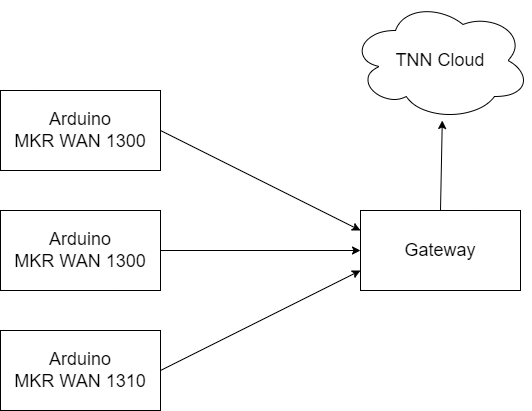
\includegraphics[scale=0.35]{Images/HW-Diagram.png}
\caption{High Level Hardware Diagram}
\label{fig:HL-HW-Diagram}
\end{figure}

Each sensor node will include an accelerometer to detect, log and transmit movement in three dimensions (x, y and z axis). This data is sent to the on-board processor of the Arduino carrier board where it is logged. The average movement on each axis as averaged and sent via data packet over LoRaWAN via a dipole antenna every hour. The carrier board itself is powered with a simple solar panel / battery setup. The pro gateway is listening for packets on the LoRa network via a mono-pole antenna. These packets are then sent to the on board Raspberry Pi 3 model B+ processor. The processor transmits these packets to the TNN cloud. This more detailed system can be seen in figure \ref{fig:HL-HW-Diagram-Detailed}.

\begin{figure}[h!]
\center
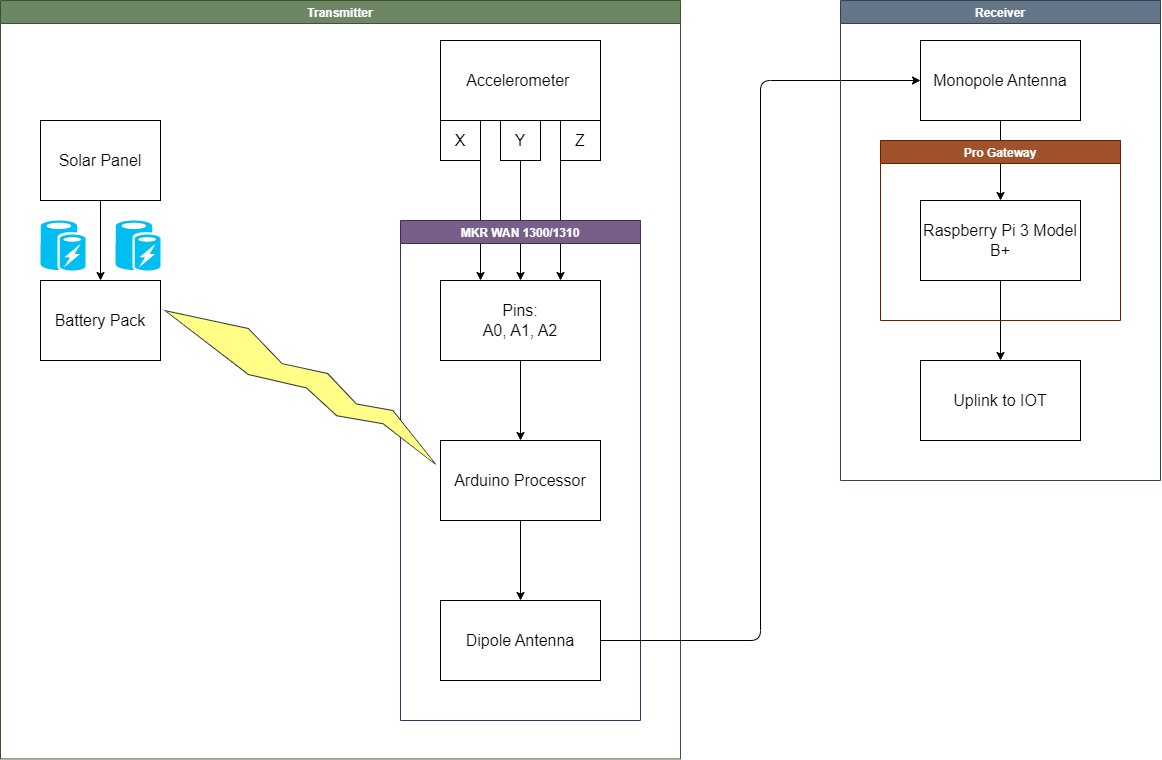
\includegraphics[scale=0.35]{Images/HW-Diagram-Detailed.png}
\caption{Detailed High Level Hardware Diagram}
\label{fig:HL-HW-Diagram-Detailed}
\end{figure}

\begin{figure}[h!]
\center
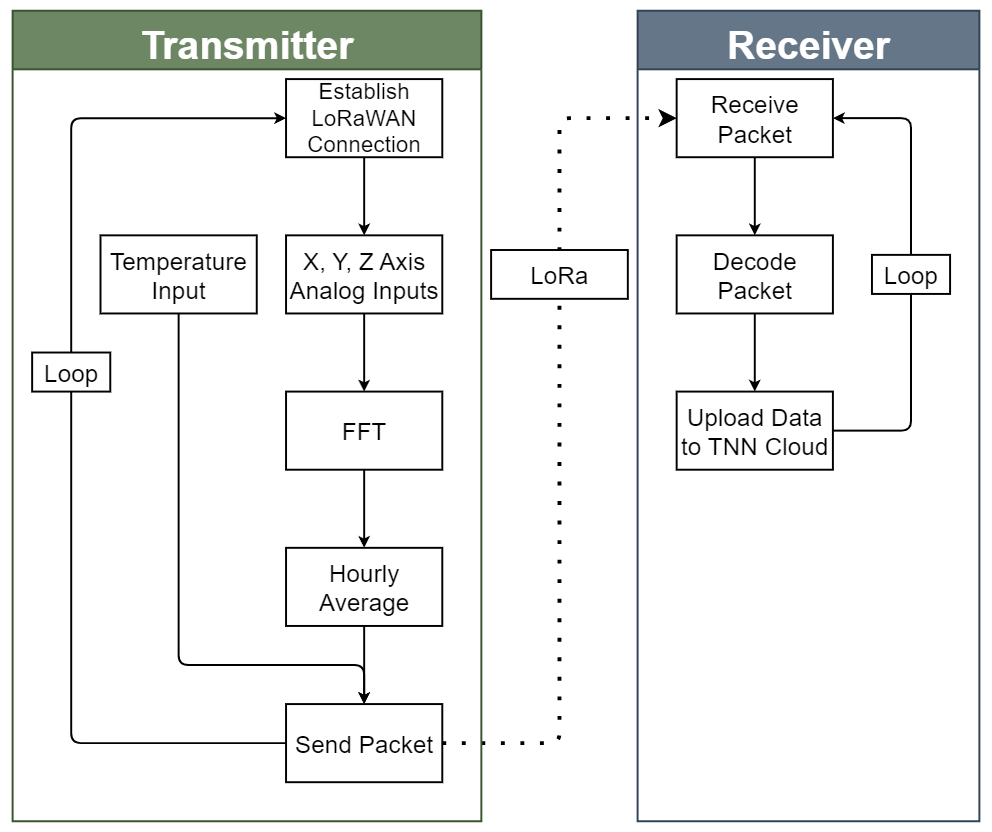
\includegraphics[scale=0.35]{Images/SW-Diagram.png}
\caption{High Level Software Diagram}
\label{fig:HL-SW-Diagram}
\end{figure}

Figure \ref{fig:HL-SW-Diagram} displays the higher level software diagram for the transceiver and receiver.  One of the major aims of the project will be to further explore this software design which is heavily dependent on the functional requirements of the system. The functional requirements of the system will  dictate the packet size and transmission frequency. Additionally, different types of windowing techniques for the Fast Fourier Transform will be explored to remove noise from accelerometer analog inputs. 




